\documentclass{nime-alternate} % Uncomment when publishing final version
% Uncomment only one of the ones below
% \usepackage{anonymize} 		   %Uncomment this line to publish
\usepackage[blind]{anonymize}%Uncomment this line for blind review
\usepackage[utf8]{inputenc}

\usepackage{float}
\usepackage{natbib}
\usepackage{graphicx}
\usepackage{todonotes}
\usepackage{etoolbox}
\usepackage[inline]{enumitem}
\usepackage{subcaption}

\begin{document}

% --- Author Metadata here. See Template---
\conferenceinfo{NIME'20,}{July 21-25, 2020, Royal Birmingham Conservatoire, ~~~~~~~~~~~~ Birmingham City University, Birmingham, United Kingdom.}
\title{Percussive Sound Generation with Virtual Listeners and Modular Synthesizers}

\label{key}
\numberofauthors{2} 
\author{
\alignauthor
\anonymize{Amir Salimi}\\
       \affaddr{\anonymize{Department of Computing Science}}\\
       \affaddr{\anonymize{University of Alberta}}\\
       \affaddr{\anonymize{Edmonton,AB,Alberta}}\\
       \email{\anonymize{asalimi@ualberta.ca}}
\alignauthor
\anonymize{Abram Hindle}\\
       \affaddr{\anonymize{Department of Computing Science}}\\
       \affaddr{\anonymize{University of Alberta}}\\
       \affaddr{\anonymize{Edmonton,AB,Alberta}}\\
       \email{\anonymize{abram.hindle@ualberta.ca}}
}

\maketitle

\begin{abstract}
Digital sound artists often require a variety of percussive samples for their music. We observed a lack of copyright-free one-shot percussive sample-packs for purposes of research and music creation. Yet for more than two decades research involving digital synthesis, genetic search, and neural networks has been used to invent and approximate novel sounds. Our goal is to generate one-shot percussive samples by leveraging modern AI technologies alongside scalable signal generation methods. Could we generate novel drum sounds through machine learning, heuristic search and modular synthesizers? We centered our approach around the combination of two central components: \begin {enumerate*} [label=(\roman*)] \item a "virtual ear" capable of learning key features of various sound groups and evaluating the proximity of unheard sounds to desired sets and \item a dynamic virtual synthesizer with a rich set of tractable parameters\end{enumerate*}. We present a generative pipeline that utilizes robust digital signal processing methods and is guided by supervised learning and genetic search towards generation of novel, high-quality, one-shot percussive sounds. We present our findings and measurements of the various approaches taken towards the implementation of the virtual ear, virtual synthesizer, and generative pipeline; hoping to expose the advantages and shortcomings of the employed methodologies and their practicality in future works via a clear demonstration of their capabilities relative to our stated goal. We also discuss and share our curated dataset of sounds along with our codebase \footnote{\url{https://github.com/imilas/Synths_Stacks_Search}} which can be used for its further expansion.


\keywords{drum, percussion, synthesis, MIR, ML, genetic, search}
\end{abstract}
% See template for CCS classification. 
\ccsdesc[500]{Applied computing~Sound and music computing}
\ccsdesc[500]{Information systems~Music retrieval}
\printccsdesc

\section{Introduction}
\subsection{Terminology}
\todo[inline,color=green!30]{I'd like to define terms such as VSTs, audio effects, Synthesizers, paramters and presets here. I throw these terms around a lot and I think some might be confused by their meaning. Is this the appropriate place for that? I'd like the reader to know these definitions before reading the intro. I can try to keep it brief and engaging}
\subsection{Background and Motivation}
The rise of Digital Audio Workstations (DAW) \cite{leider2004digital} and Virtual Studio Technology (VST) based plug-ins \cite{tanev2013virtual} have rapidly transformed the sonic and material landscape of music production in the recent years. Coupled with this rise in popularity is a vast array of commercial products and services dedicated to satiating the need of amateur and professional music producers for unique sounds; most commonly via audio samples: one-shot drum samples, long sustained notes (commonly referred to as pads or textures), and loops (percussive or melodic) are common deliverables. Two notable examples of these commercial services are \textit{loopmasters}\footnote{loopmasters.com} and \textit{splice.com}\footnote{splice.com}. Furthermore, VST plug-ins can emulate complex audio synthesizers and effects which some producers may find daunting or time consuming to work with from scratch. In many cases VST plug-in vendors or unaffiliated enthusiasts sell additional presets for these plugins, targeted towards producers who do not have the time or interest in creating their own. Producers may further modify these presets until their desired sound is reached.\\
Our work is motivated by the idea of finding new, convenient methods for the expansion of a music producer's library of sounds. Primarily with generation of novel, one-shot audio samples but also with automated search and creation of presets for virtual synthesizers that a producer might find  interesting. Using the generation of short, percussive audio samples as a starting point this project is a proof of concept for promising avenues towards our motivational goal.\\

\subsection{Methodology}
Towards our goal of generating original audio, we found the proper implementation of 2 major components to be crucial:
\begin{itemize}
    \item \textit{Virtual Synthesizer}: A flexible, deterministic, and tractable generator which can create audio. The core of our implementation made use of pippi, \footnote{https://github.com/luvsound/pippi} a fast, offline focused python DSP library with a C backend. We additionally used the scipy\cite{jones2001scipy} library a few audio effects that we found lacking in pippi. 
    \item \textit{Virtual Ear}: An ear that returns an evaluation of an audio sample; estimating the effectiveness of an audio sample's fulfillment of a producers requirements. The ear's evaluation guides the generation process towards a desired path, making the implementation and training of the ear crucial to the sounds which are generated. A particularly effective implementation was done by using a labeled set of percussive and non-percussive audio files to train a custom model (combination of a simple Convolutional Neural Net (CNN) and a custom envelope estimation algorithm), giving us a "virtual drum detector ear". \\
\end{itemize}
Our components are designed with modularity and parallelizability in mind. This allows each component to be debugged, modified, and improved without requiring modifications in other components; additionally increasing the scalability and speed of experiments.
Section \ref{impl} contains further discussion of the components as well as the code that glues the project together.\\ 
While the main focus of this project is the generation of novel percussive sounds our methodology indicates promising results with regards to creation of new presets for any virtual synth without the need for a-priori knowledge of the functions or its parameters (i.e the effect of parameter modulation on the sonic output). We also demonstrate the viability of a few lesser explored avenues for the purposes of audio synthesis and Music Information Retrieval (MIR), notably:
\begin{enumerate}[label=\roman*]
\item Heuristic search methods for the creation of new presets for virtual synthesizers. More concretely, we observed that given a virtual ear which could reliably score pieces of audio based on its resemblance to a desired category (e.g: kicks, snares, piano) we were able to rapidly search the parameters of a virtual synthesizer and create numerous parameter-sets (i.e presets) which resemble our desired category of sounds.
\item The viability of virtual synthesizers based on Digital Signal Processing (DSP) methods for fast, unsupervised creation of novel audio, discussed in more detail in section \ref{related}. \\
\end{enumerate}

\subsection{Related Work and Contradistinctions}
\label{related}
Numerous deep, neural network models have been proposed and utilized for the purpose of signal generation in recent years. WaveGans and WaveNet have been subject to significant improvements and experiments since their proposal \colorbox{green!=40}{\cite{nsynth2017} + Many more references to be added.} Even more recently Variational AutoEncoders (VAE's) have been utilized for generation of short percussive samples \cite{aouameur2019neural,ramires2019timbfeat}. In this work however, we opt to use digital signal processing methods to create a virtual synthesizer for the generation of audio signals as it provides several unique advantages:
\begin{enumerate}[label=\roman*]
  \item Fast, offline rendering of audio with no reliance on GPU: Currently not possible with state of the art models such as parallel WaveGan \cite{yamamoto2019parallel} and parallel WaveNet \cite{oord2017parallel}. 
  \item Rendering at high sampling rates: Performance speed being a common issue, the standard sampling rate in most audio generation work utilizing neural networks appears to be under 24 khz \cite{yamamoto2019parallel,oord2017parallel,aouameur2019neural,ramires2019timbfeat}. However, a significant number of untrained human ears can detect a change in quality of audio between sampling rates of 192 khz and the industry standard of 44.1 khz \cite{reiss2016meta} with a dramatic increase in quality detection after training. Therefore we can safely assume that most producers would prefer their audio samples to have sampling rates of 44.1 khz or higher. 
  \item Neural networks are often viewed as unexplainable black box solutions. Some models such as VAE's can learn an underlying latent space of parameters and capture the "essence" of the different labels in a dataset. However, these spaces are learned in an unsupervised manner and must be manually analysed, perhaps extensively, before they can be understood \cite{esling2018generative}. The use of a virtual synthesizer for audio generation makes our parameters readily understandable and easily modifiable. \\
  
\end{enumerate}
Automatic programming of virtual synthesizers has also been a topic of interest. In early 2000s, Interactive Genetic Algorithms (IGA's) were utilized for the generation of new sounds with various sound-engines \cite{johnson1999exploring,dahlstedt2001creating}. More recent work by Yee-King et al. \cite{yee2018automatic} used LSTM and genetic algorithms to find the exact parameters used to create a group of sounds. The sounds approximated were made by the same virtual synthesizer, not an external source; making the eventual replication certain even with random search. Since this work more focused on pads and textures rather than drums, feature matching in this also appears to not be concerned with the envelope of the sounds but rather the frequency content within arbitrary time windows. Yet another recent, impressive work by Esling et al. used a large dataset of over 10,000 presets for a commercial VST synthesizer to learn a latent parameter space which can be sampled for creation of new audio \cite{esling2019universal}. As stated before, our work presents a rapid approximation of percussion sounds with no previous knowledge about the sonic capabilities of our virtual synthesizer, exploring the actual parameter space rather than its latent representation. 


\subsection{Data And Project Replication}
\label{data}
Our data is a large set of drum samples aggregated from personal libraries, free drum kits from sampleswap \footnote{https://sampleswap.org/} which we further processed to suit our categories, and a large set of drum sounds aggregated from royalty free sources such as musicradar \footnote{https://www.musicradar.com/}. We will make our dataset of free-drum sounds available for download. The scripts used to download and process royalty free samples will also be made available. Further information about downloading our dataset can be found on the project's github page. \\
Our drum categories are claps, hats, kicks, rims/other, shakers, snares, mid-toms and high-toms. Other categories are chopped guitars, chopped pianos and stacks (randomly generated synth noise), utilized for learning percussive vs not-percussive sounds. Some notes about our dataset:
\begin{itemize}
\item Of the 6000 drum-sounds utilized in our work, the kick, snare and hat categories have the largest share at around 20\% each, while the shaker and rim (other) categories have the smallest at 5\% combined. Due to this we only focused on learning from kicks, snares, toms, claps and hats for Phase 1 of training \ref{sec:ear}.
\item For Phase 2 of training we only focused on categorizing snares, claps, kicks, hats and other (percussive sounds such as shakers, rims and unusual percussions that we couldn't categorize were grouped into this category). 
\item In order to offset bias from data imbalance during training of our models, the categorical cross entropy loss was weighted by the category sizes. 
\item For training any given model, 80\% of our data is used for training the models and 20\% is used for testing. 
\item We limit the size of the stack category to 50\% of the total size of our drum dataset. This is done in order to measure whether the features extracted can address the "Open Set Recognition" problem, which will be discussed further in section \ref{sec:ear}.
\end{itemize}
\section{Implementation}
\label{impl}
\subsection{Virtual Synthesizer}
We used the python based Pippi library for sound generation\footnote{https://github.com/luvsound/pippi}. This library uses a C back-end and focuses on fast offline generation of audio signals. In our implementation a synthesizer can have any number of sub-modules. The parameters that deterministically dictate the output signal of the sub-module as well as the range of values each parameter can take are shown in table 1 \ref{table:1}. We call this number the \textit{stack size}. For the range of parameters each sub-module can take we call the sets of parameters that characterize a synth's sub-modules a \textit{program} (analogous to a preset).  Each sub-module can make an audio signal with the length of 0.1-1 second. If a Synth has a stack size of more than 1 these audio signals are overlapped and the total amplitude is normalized.\\
\begin{table}[h!]
\centering
\resizebox{\columnwidth}{!}{\begin{tabular}{ |c|c|c| } 
\hline
Parameters & Value Range & notes and constraints\\
\hline \hline
Attack & 0-3 & A-D-S-R values relative\\
Decay & 0-3 & relative to A-S-R\\
Sustain & 0-3 & relative to A-D-R\\
Release & 0-3 & relative to A-D-S\\
OSC type & sine,square,saw & tone type\\
IsNoise & boolean & whether to generate noise\\
Sample Length & 0-1 second & - \\
StartTime & 0-1 second & Length+Start<1\\
Amplitude & 0.1-1 & 1 = max amplitude\\
Pitches(notes) & list of pitches &  range of C0(16.35hz) to B9 \\
HP filter Cuttoff & 0-20000 & -\\
LP filter Cuttoff & 20000-HP & never lower than HP cutoff\\
Filter Order & 4,8,16 & butterworth filter order \\
\hline
\end{tabular}}
\caption{Synthesizer Sub-module Parameters. Despite the simplicity of the parameters and our efforts at constraining the ranges, the number of parameters that can be randomly chosen for each sub-module is in the order of $10^{15}$ }
\label{table:1}
\end{table}
\begin{figure*}[h]
\centering

\begin{subfigure}[b]{\linewidth}
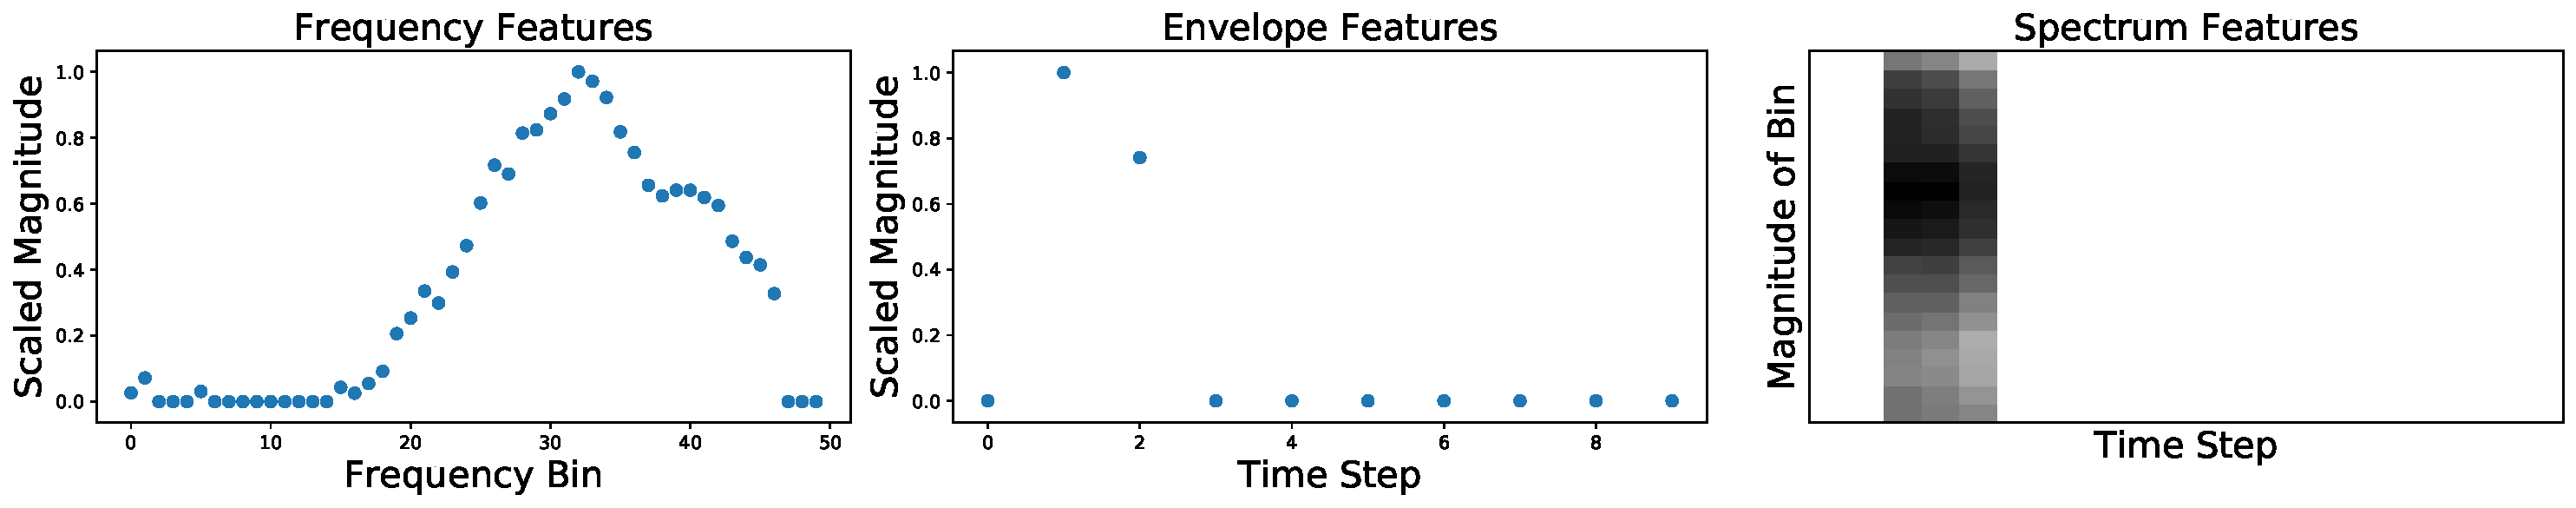
\includegraphics[width=1\linewidth]{images/ff1.pdf}
\caption{Organic hat sample}\label{fig:64stack}
\setcounter{subfigure}{1}%
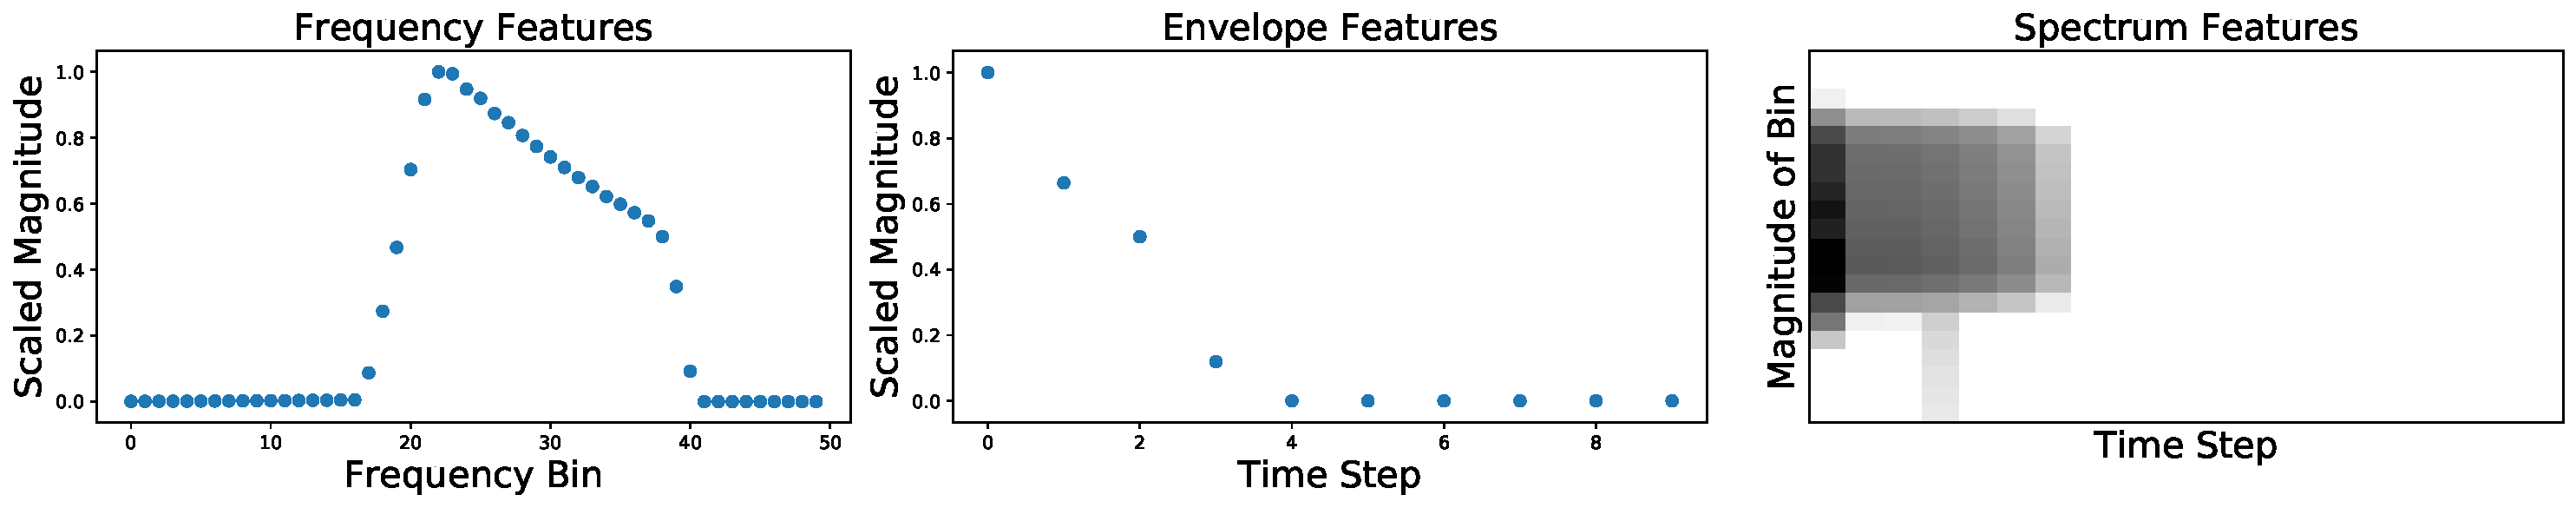
\includegraphics[width=1\linewidth]{images/ff2.pdf}
\caption{Randomly generated audio with percussive qualities, resembling a tight snare}\label{fig:64stack}
\setcounter{subfigure}{2}%
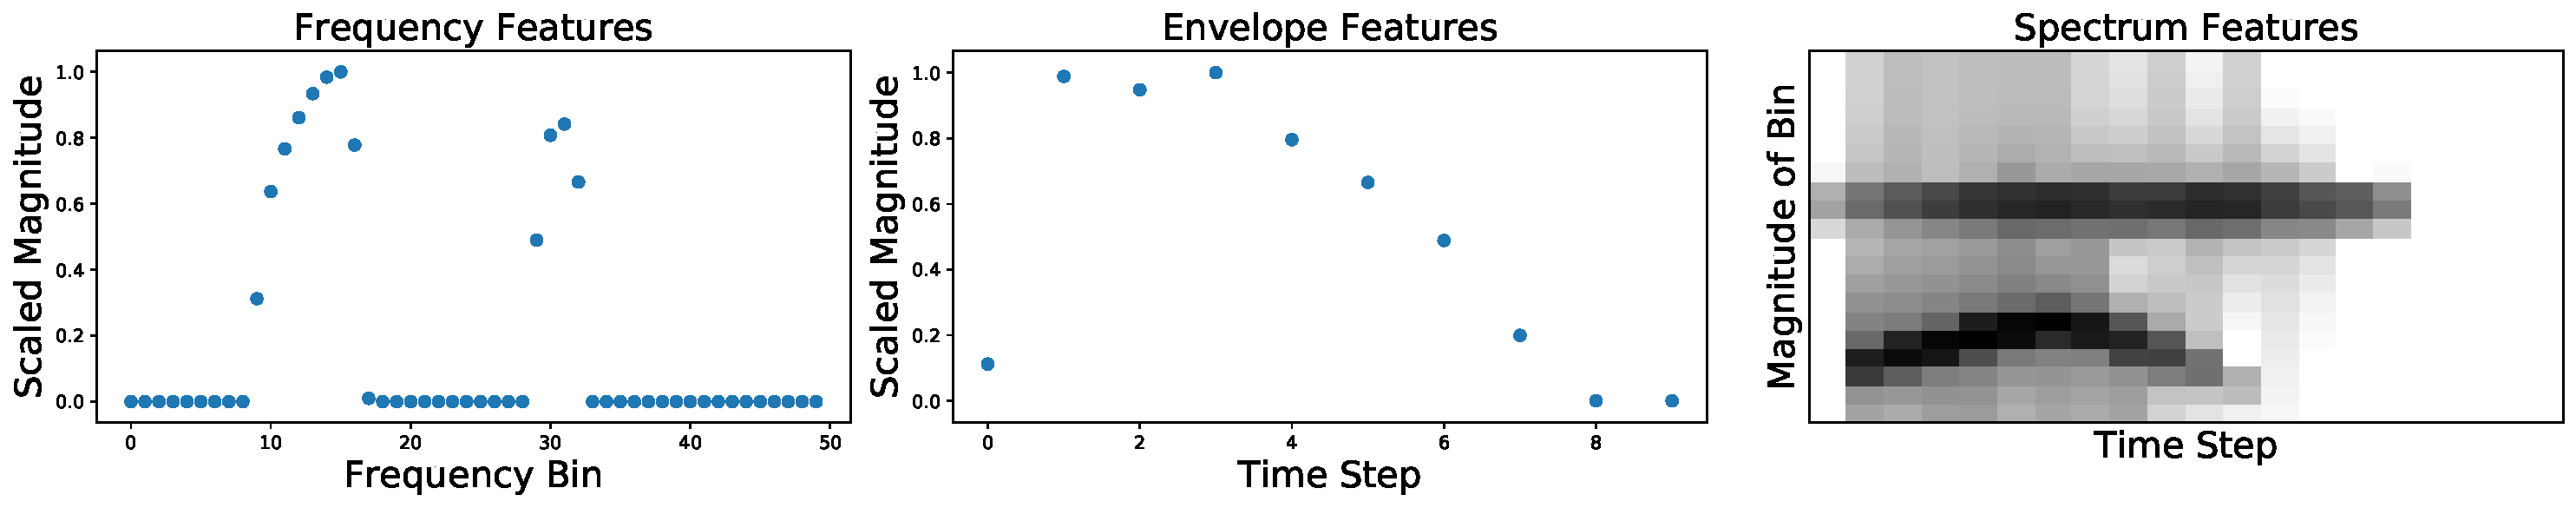
\includegraphics[width=1\linewidth]{images/ff3.pdf}
\caption{A randomly generated noise with a percussive envelop but non-percussive frequency features (modulated pitch)}\label{fig:64stack}
\setcounter{subfigure}{2}%
\end{subfigure}

\caption{Graphed representation of features extracted for 3 different samples. Sample $a$ is an organic hat from our database. sample $b$ is an example of randomly generated noise with percussive qualities that we found suitably similar to a snare sound. Sample $c$ is an example of a randomly generated noise where the spectrum features are necessary for proper classification.}
\label{fig:stackspectrums}
\end{figure*}

\subsection{The Ear}
\label{sec:ear}
\subsubsection{Feature Extraction}
What we refer to as an "ear" is any method of evaluating a piece of audio and capable of "listening" to a piece of audio and giving it a score (or a list of scores) based on how well it satisfies certain criteria. Since in this work we are mainly focused on percussive generation what we require from the ear is to give us probabilities of an audio sample belonging to various categories. As our synthesizer outputs are deterministic for all programs the ear's evaluations would allow us to associate the categorical probabilities of each sound with the program that generated it. In section \ref{gens} we discuss how these scores were used for navigation of our synthesis towards parameters which give us the desired sonic output.\\
 With our dataset \ref{data} of labeled drum sounds we can confidently categorized unlabeled drum sounds given that we know they are drum sounds. However, a major hurdle towards the implementation of a "drum from non-drum" recognizing ear is that the set of sounds that are not percussive is infinite. Since we can represent different drum groups using our categorized data (closed set), but effective aggregation and feature extraction of non-drum sound data is not practical. We hypothesize that $Task\,1$ falls within the domain of "Open Set Recognition"\cite{scheirer2012toward}. "Open Set Recognition" problem arises when a set that is being categorized has practically infinite diversity, often making learning-by-example impossible without further domain knowledge. While ML techniques can be effective with classification of a closed set of examples, the classification of an infinite set cannot be reliably achieved with current ML methodologies\cite{geng2018recent,mundt2019open}. \\
  In our case, as discussed in section \ref{survey}, the majority of sounds generated by the synth do not resemble percussion. Even if we only consider 1 second long sounds made with a single stacked synth, the set of synthesizer parameters (and we assume, the sound generated by these parameters) is extremely large. In our case, we determined that there are 2 steps necessary to effectively extract percussive sounds from the randomly generated noise from the virtual synthesizer: 
  \begin{enumerate}
   \item  $Phase1\,1$: Binary separation of sounds with percussive features from non-percussive sounds.
   \item $Phae2\,2$: Given confidence that the sound being categorized is percussive, categorizing the type of drum or percussion.
 \end{enumerate}
We are interested in extracting generalized features that can be applied in other audio domains. In this work we rely entirely on Fast Fourier Transform (FFT) and by extension Short-time Fourier Transforms (STFT) for feature extraction. Using FFT a signal can be represented by a vector with each index corresponding to a frequency-bin (a range of frequencies too close to be distinguishable) and the value at each index corresponding to the combined-magnitude of the frequencies within the bin. STFT can be employed when a more accurate representation is desired; via the application of the FFT to a sliding time-window on the signal to create a matrix (a list of vectors). This matrix can effectively represent the frequencies present in the signal at each time step, given the right window-length and hop-size (how much the window is shifted at each time-step).\\
Various works have demonstrated effective reconstruction of signals given their STFT \cite{nawab1983signal,griffin1984signal}. The loss of phase information may be an issue in some domains \cite{sturmel2011signal}, however, phase information has little impact on the human auditory experience. If the original signal can be otherwise accurately reconstructed from its STFT, perhaps further transformation and analysis of the STFT may be relied on as source of fundamental features necessary for audible signal categorization. Following this and in the interest of keeping the feature space small and fundamental, other methods of feature extraction which have proven effective at instrument and percussion categorization such as Spectral-Centroids \cite{schubert2004spectral} and Zero-Crossing Rates \cite{gouyon2000use} are not utilized.\\
Using only the STFT of signals as source of feature extraction we defined 3 transformation functions which we believe to capture important, unique attributes of percussive sounds. These functions were applied at training time to 1 second audio samples before being sent to a classifier. 
\begin{enumerate}
\item Envelope Transformation: The goal of this feature is to capture the changes in loudness for the duration of the signal. Using STFT we generate a matrix $M_{i \times j}$ with rows $i$ and columns $j$ corresponding to time steps and frequency bins respectively, and with values $v_{i \times j}$ indicating the magnitude of the frequency bin $j$ at each time-step $i$. Information about the envelope of the signal can be extracted by summing the values of $M$ for each time-step (or row $i$), giving us a feature vector $v_i$. This vector is then normalized to the range of 0 to 1. The information contained in this vector is similar to that of a Root-Mean-Square measurement.
\item Frequency Transformation: A static, normalized snap-shot of the the frequencies present within the audio. The calculation of this feature vector is similar to the envelope, but the summation is done along the frequency axis. Another important distinction is that since capturing an adequate frequency resolution is important for this transformation, we utilized shorter hop-sizes and wider windows. A Mel Scale transformation was also applied in hopes that the captured features better represent human perception of frequencies. 
\item Spectrum Transformation: This function is simply a Mel Scaled STFT with its values normalized from 0-1. Since this features is a 2D matrix rather than a vector it captures more information about our signal but requires heavier, more complex computational methods to be utilized. 
\end{enumerate}   
\subsubsection{The Models}
Using the described features, we trained several models for Phase 1 and 2. These include Fully-Connected (FC) models, Convolutional Neural Nets (CNNs) and CNN + Long Term Short Memory models (CNNLSTM). The task of Phase 1 is to separate drums from not-drums (DrumVsNotDrum, or DVN). The task of Phase 2 is to categorize drums and percussion (DrumVsDrum, or DVD). We kept our feature space small, making it viable to for the task of designing models and picking the right features being done on a trial and error basis. A summary of models utilized in our pipeline is given below:
\begin {enumerate}
\item FC-DVN: A small fully connected network trained on Envelope features, reaching 97\% accuracy on our test data for Phase 1. 
\item CNNLSTM-DVN: A combination of CNN and LSTM models, where the CNN model extracts higher level features that are fed temporally to an LSTM cell. This model is trained on spectrum data and reaches 98\% accuracy on our test set for Phase 1.
\item E+F-DVD: A fully connected model trained on a concatenation of envelope and frequency features for Phase 2. Reaching 80\% accuracy for 6-way drum categorization.
\item CNN-DVD: A deep CNN model that reaches used for Phase 2. 82\% accuracy in a 6-way drum categorization. Trained on Spectrum features.
\item FC-DVD: Fully connected 3 layer neural net with 78\% accuracy for 6-way drum categorization. Trained on Spectrum features.
\end{enumerate}
The number of parameters for these models were picked rather arbitrarily. We'd like to note that based on our anecdotal observations the minor modifications in features played a much more significant role in the model accuracy than major parameter changes. Also as discussed in section \ref{survey}, despite it's marginally lower accuracy rate, the FC-DVD model has a slight but noticeable advantage in regards to matching human categorization of data. Likewise, Freq+Env had a much lower degree of agree-ability with humans despite its better performance on organic drum data, leading us to believe that model accuracy on test data alone cannot be relied upon when the domain of sounds being categorized is switched from organic samples to a virtual synth. \\
With our models showing efficacy at categorizing organic drums vs randomly generated synth sounds, and categorizing organic drums accurately, we combine models in order to increase the efficacy of each phase and address the "open set" problem for our task. For Phase 1 we only determine sounds as percussive if both FC-DVN and CNN-LSTM have determined it as such with over 90\% confidence. For the majority of our random generations that is not the case, but if a randomly generated sound is passed this phase, our three categorizers assign their categorizations to this sound. These categorizers have a moderate degree of agree-ability as seen in \ref{survey}, but often there is not an unanimous decision. The Fourth method of categorization, "averaged-cat", is implemented by taking the sum of the softmax outputs of all three categorizers and use this sum to determine the category. \\
These models can be combined and weighted in various ways. The confidence thresholds can be modified in order to implement "ears" with different properties. A glaring issue in the current implementation is the treatment of softmax outputs as a reasonable measure of a models confidence. For various reasons some models tend to have much higher confidence in their scores, skewing attempts at finding a consensus. 

% How Can The Synth and Ear Interact?
%
\subsection{How Can The Synth and Ear Interact?}
With our Synth and Ear in place we can quickly generate programs for our Synth, create the corresponding audio sample and get the scores for the audio sample. If the ear returns a vector of categorical probabilities, we can assign categorical ranks to the audio sample. For example, the category with the highest probability will have the rank of 1, second highest would rank 2nd, and the lowest probability will have the rank of n (assuming n categories).\textbf{
But how can we use this to create percussion sounds?}\\\\
We utilize our tools in three different methods of generation, with their specific implementation discussed in section \ref{gens}.
\begin {enumerate} [label=(\roman*)]
\item Random Generation: We randomly create a drum program until a sound belonging to our category is produced. We hypothesize that due to the speed of our experiments it is a viable approach.
\item Multivariate Distribution Sampling: We attempt to learn the joint distribution of our parameters in order to maximize generation of a certain drum category. 
\item Genetic Search: We treat our parameters as genes and attempt to use evolutionary search algorithms to find programs that the ear deems most fit.\\
\end {enumerate} 
\todo[inline,color=blue!30]{As seen in Figure \ref{fig:rank portions}, there is a bias in random generation towards making higher ranking hats and kicks and lower ranking shakers and claps. Is this bias because of Synth structure or a problem with the ear? Will analyse further after updating ear}

\section{Novel Generations}
\label{gens}
\subsection{The Goal}
 Our goal is to rapidly create high quality, novel drum sounds. In this work we analyze random generations in a build-up towards a guided generation via heuristic search.
\subsection{General Methods}
\subsubsection{Random Generation}
To establish a benchmark we seek to assess the likelihood of generating samples of each category if we generate programs for various stack sizes by random selection of parameters. We have observed a bias in generations as indicated in figure \ref{gens}.\\
\subsubsection{Evolutionary Search}
We implemented evolutionary search using DEAP \citep{DEAP_JMLR2012}. A parameter set is assumed to be an individual with each parameter being its genes. To measure an individuals fitness we use the formula $fitness=score-rank$. As generations evolve, a Hall-of-Fame (HOF) list with a fixed size tracks the best individuals to ever live in any given generation, updating itself after each batch of off-springs is evaluated.\\
To ensure diversity of the HOF individuals the fitness score should also consider some measure of uniqueness. A weighted minkowski distance \footnote{https://docs.scipy.org/doc/scipy/reference/generated/scipy.spatial.distance.minkowski.html} between the genes of an offspring and the HOF individuals may be a good measurement.\\
A generation of $N$ individuals are initialized randomly. To create the offspring generation, each generation goes through mutations and in-place gene crossovers. The new generation consists of the top 80\% of the offspring generation and 20\% new individuals to quicken gene diversity. If the new individuals are coming directly from previously measured high scoring parameter sets, we ensure that they cannot be directly added to HOF without going through mutations and crossovers first.\\
\subsubsection{Survey of Generated Drums}
\label{survey}
\begin{figure}[H]
\centering
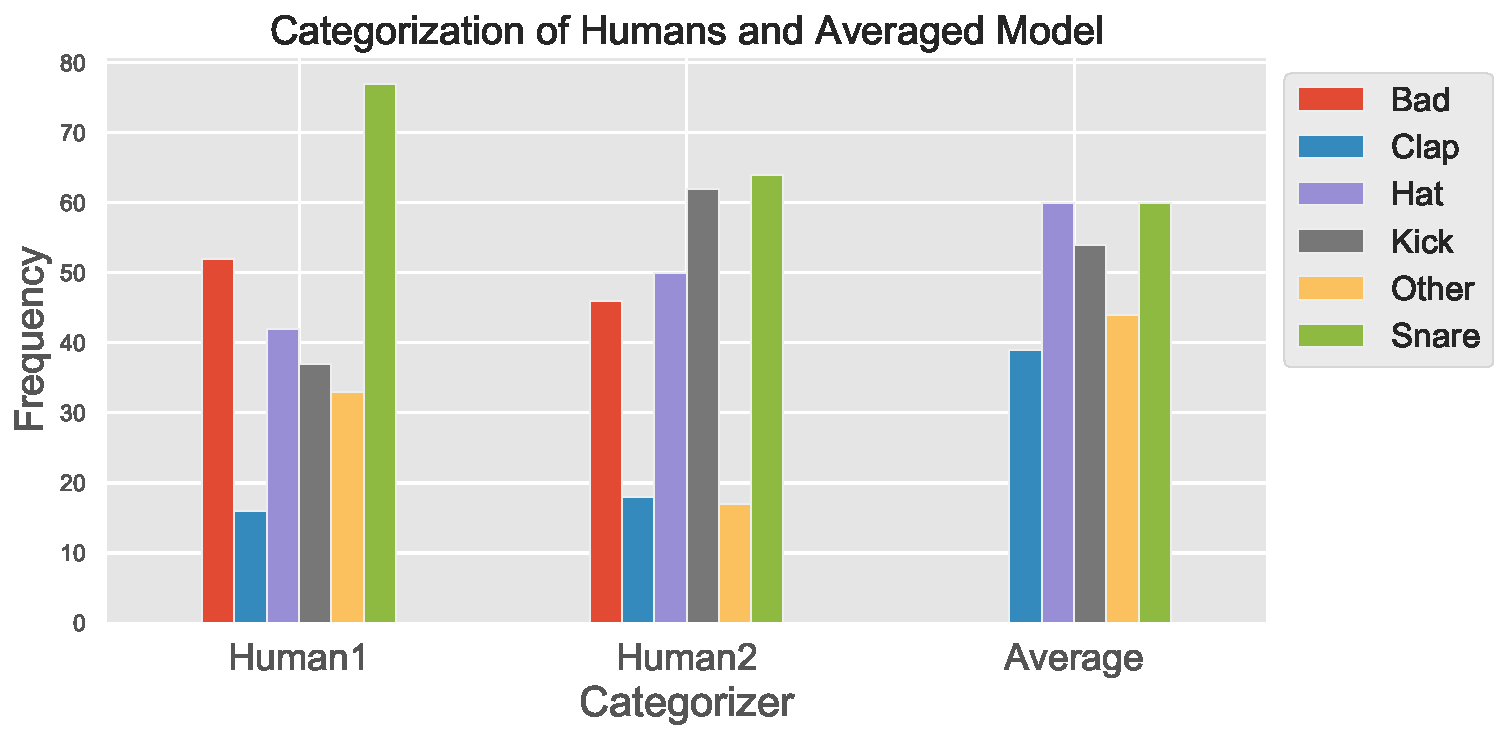
\includegraphics[width=1.1\linewidth]{images/cat.pdf}
\caption{Frequency of assigned labels for the human categorizers and the average categorizer}
\label{fig:freq-survey}
\end{figure}

To measure the quality of the samples produced by our pipeline and the power of our models, we randomly generated around 50-60 samples in the following categories: "snare","kick","hat","clap" and "other" (combination of rims, 
shakers and unusual percussive sounds"). These samples were determined to be percussive and then categorized by 4 different models (FC, CNNLSTM, E+F and AVG). We ensured a balanced division between samples of stack sizes 1,2 and 4 (each stack is responsible for a third samples under each category). Both writers then categorized these samples without knowledge of other categorizations (human or computation models). It's important to note that:
\begin{itemize}
    \item Humans had an additional category of "bad" for samples that they deemed not percussive. The "bad" category indicates that the sample should have been skipped in phase 1. 
    \item With 6 categorization groups, human's had the same categorization in 47\% of cases
    \item The agreement between the humans and AVG was 44\% and 47\%, not significantly lower than agreement with each other. 
    \item Of 257 samples, both humans agreed with FC, CNNLSTM, AVG and E+F respectively in 78, 76, 76 and 46 of cases.
\end{itemize}
We assess the reliability of agreement between humans and categorization models via the Fleiss' kappa coefficient \cite{fleiss1971measuring}. The value of 0 or less for this coefficient indicates no agreement beyond random chance, and the value of 1 indicating perfect agreement. Our kappa measurements \ref{kappa_table} lie within the 3.5-4.5 range, indicating mild to moderate agreement between humans and machines. We again measure this coefficient after dropping samples that were categorized as "bad" by the authors, as samples that humans deem to be "bad" indicate a failure in phase 1 and arguably should not have been categorized by the models at all. Dropping of samples that both authors deemed "bad" causes 8\% reduction of our data (21 samples) and a small increase in kappa score. Dropping samples either reviewer deemed bad resulted in a 30\% reduction of samples and relatively large increase in kappa scores. \\

Possible takeaways from this survey:
\begin{itemize}
    \item The survey brings into question the reliability of our phase 1 models, as 30\% of the generated samples were deemed not percussive by at least 1 reviewer and 8\% by both reviewers
    \item The task of categorizing synthetic drums is difficult. Survey shows that the scale of agreement within humans as well as between humans and various model combinations is moderate at best, even after removal of "bad" samples.  While the same models can easily achieve 98+ percent accuracy when tested on organic drum samples. This may be a manifestation of the "open set recognition" problem. 
    \item While there is much room for improvement, our pipeline can generate and categorize drums and percussive sounds with a promising degree of success. 
\end{itemize}
\begin{center}

\begin{table}
 \resizebox{\linewidth}{!}{\begin{tabular}{||c c c c c c c||} 
 \hline
 Drop Bad? & Size & HvH & H+FC & H+CNN & H+ALL & 3 models \\ [0.5ex] 
 \hline
 No & 257 &0.37 & 0.35 & 0.35 & 0.36 & 33\\ 
 \hline
 if both & 236 & 0.31 & 0.37 & 0.37 & 0.38 & 33 \\
 \hline
 if either& 180 & 0.47 & 0.50 & 0.48 & 0.46 &  0.37 \\
 \hline
\end{tabular}}
\caption{\label{kappa_table}Table of Fleiss' kappa coefficient to measure the degree of agreement between humans (HvH), humans with FC model (H+FC), humans with CNNLSTM model, humans with all models (H+ALL), and the 3 models }
\end{table}
\end{center}

\section{Summary and Conclusions}

\begin{itemize}
    \item Our methodology was successful in generating novel examples of some percussion categories.
    \item Reiterate the importance of ear.
    \item There are potential benefits (e.g: pedagogical, software engineering, efficiency, data search, generality of solution, etc.) to separate some audio generation tasks into multiple parts, rather than throwing everything at some neural net. 
    \item With the right implementation of DSP methods to create a synth, Genetic search (viewed as too slow by previous work) is viable for finding  desired programs and parameters.
    \item Neural nets are function approximators. You don't need them if the actual function is understandable and simple...(but is our task simple enough? how do I prove it?)
    \item When possible, using DSP methods instead of NNs is preferable in many ways(speed,computation,hardware requirements).\\
    \colorbox{green!=30}{Include some speed measurements in appendix?}
    \item ...
\end{itemize}
\section{Future Work}
\begin{itemize}
    \item Potential for other generative methods (e.g reinforcement learning)
    \item Making the synth's sound range more diverse while maintaining speed and efficiency
    \item Can our approach be used for VSTs?
\end{itemize}

\section{Ethical Standards}
We affirm that our work follows the principles of ethical and professional conduct. No drums were harmed in the making of this paper.
\bibliographystyle{abbrv}
    \bibliography{nime-references} 
\end{document}
